\documentclass[]{beamer}

%Package declarations
\usepackage[utf8]{inputenc}
\usepackage[spanish]{babel}
\usepackage{natbib}
\usepackage{graphicx}

%Theme related configurations
\usecolortheme{seahorse}
\usetheme{Berkeley}

% \graphicspath{..\Docs}



%Title of the presentation
\title{Instrumentación electrónica avanzada cómo oportunidad para la automatización de sistemas de producción de alimentos en áreas del corredor seco.}
\author{Luis Guillermo García Ordóñez}
\date{10 de Noviembre 2018}



\begin{document}
\maketitle
\section{¿Qué es el corredor seco?}

\begin{frame}{¿Qué es el corredor seco?}

\note{Desde un punto de vista ecológico}
Es una zona de bosque tropical seco que presenta un patrón de lluvias irregulares, caracterizado por extensos períodos de sequías reduciéndose hasta 30\% y 40\% durante el período del niño.
\begin{figure}
    \centering
    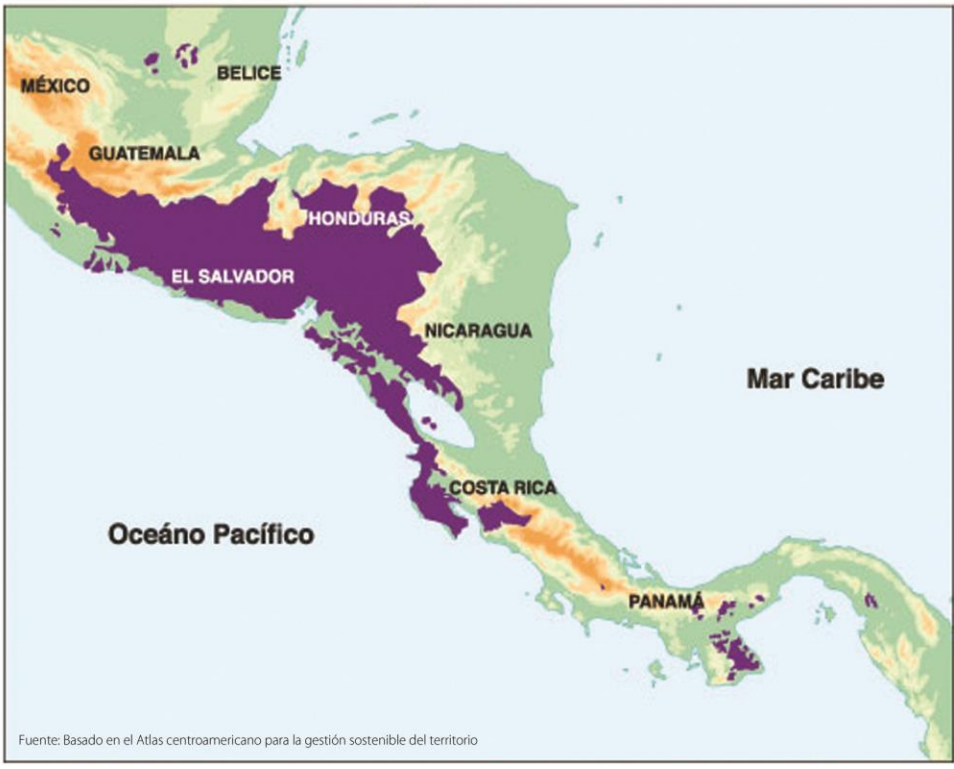
\includegraphics[width=0.5\textwidth]{Docs/Mapa_CS}
    \caption{\small \textit{Dry Corridor Central America}, Situation Report, June 2016, \textbf{FAO}}
    \label{fig:my_label}
\end{figure}
\end{frame}

\begin{frame}{}
\begin{figure}
    \centering
    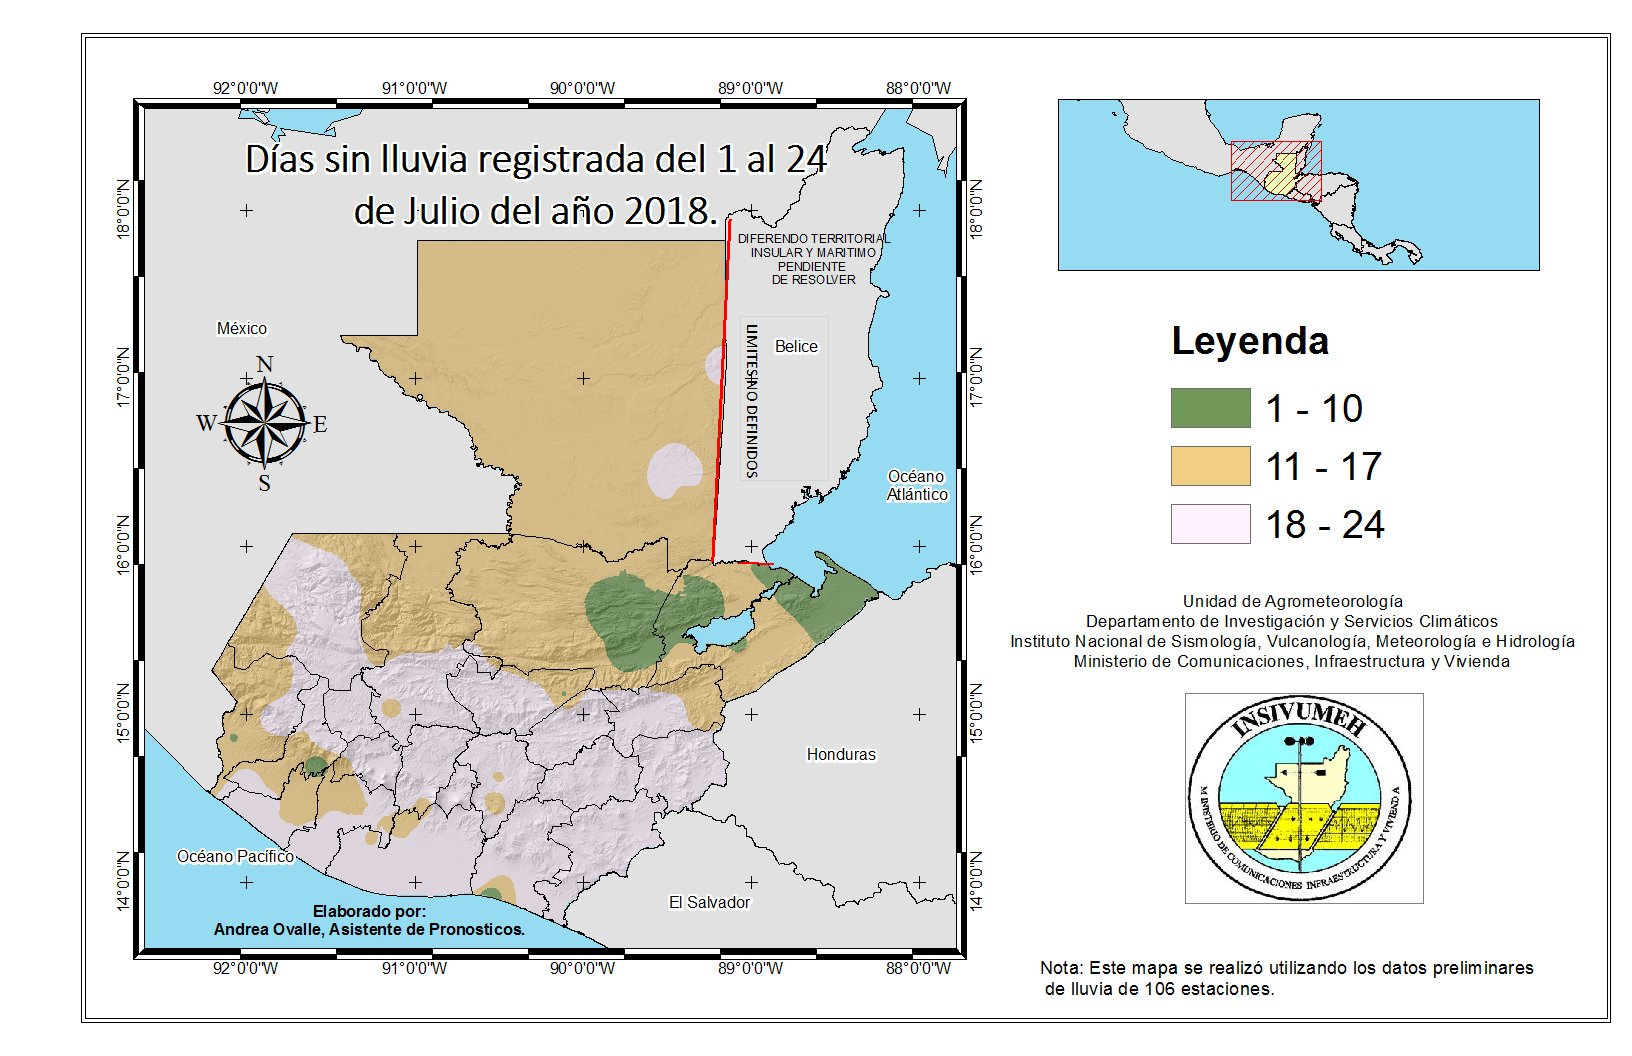
\includegraphics[width=0.9\textwidth]{Docs/diassinlluvia}
    % \caption{Caption}
    \label{fig:my_label}
\end{figure}
\end{frame}

\begin{frame}{La crísis en números}
    \begin{figure}
        \centering
        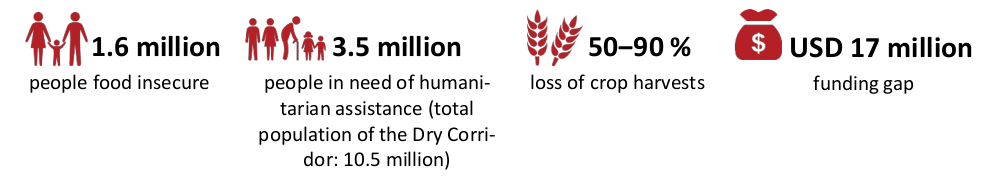
\includegraphics[width=0.8\textwidth]{Docs/cs_in_numbers}
        \caption{Cífras estimadas en centroamérica;  FAO, \textit{Situation Report}, Junio 2016}
        \label{fig:my_label}
    \end{figure}
    \begin{itemize}
      \item Durante la época de lluvias, la primera temporada de producción de maíz y frijol contribuye en 60 y 35 porciento, respectivamente, a la producción total anual.
      \item 1.5 millones de personas necesitan ayuda humanitaria en el 2016. %FAO Situation Report 2016
      \item 175,126 hectáreas de cultivo (maíz, frijol) perdídas en el 2018. %FAO GIEWS UPDATE
      \item 1,290,785 Personas afectadas en Guatemala. %FAO GIEWS UPDATE
    \end{itemize}
\end{frame}

\begin{frame}{¿Cómo mitigar este problema?}{La respuesta de la FAO en el 2016}
      \begin{itemize}
        \item Implementación de un sistema de emergencia  para beneficio de 7000 famililas.
        \item Creación de un fondo de emergencia y actividades de rehabilitación (SFERA) exclusivo para el corredor seco.
        \item Implementación de un programa de respuesta para fortalecer las capacidades de manejo de riesgo a nivel nacional promoviendo buenas prácticas y \textbf{nuevas tecnologías}, reduciendo el impacto del clíma extremo.
      \end{itemize}

\end{frame}

\begin{frame}{¿Qué nos espera?}{Algunos escenearios para el 2030}
  \begin{figure}
     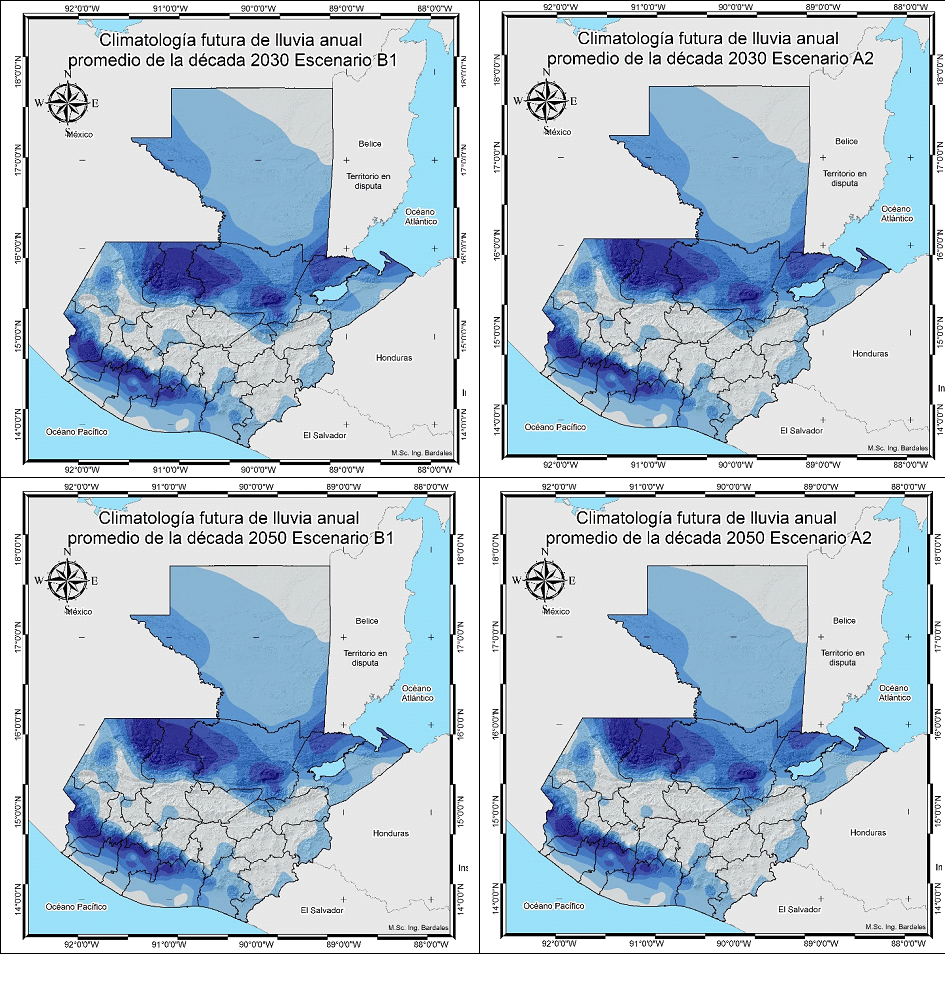
\includegraphics[width=0.6\textwidth]{Docs/Predictions}
    \caption{Presipitación promedio anual estimada para el 2030 según distintos modelos \emph{Fuente: INSIVUMEH}}
    \label{Fig:Lluvias2050}
  \end{figure}
\end{frame}

\section{La Electrónica como posible solución}
\subsection{Electrónica Aplicada a la agricultura}

\begin{frame}{La electrónica como posible solución}
  \begin{figure}
    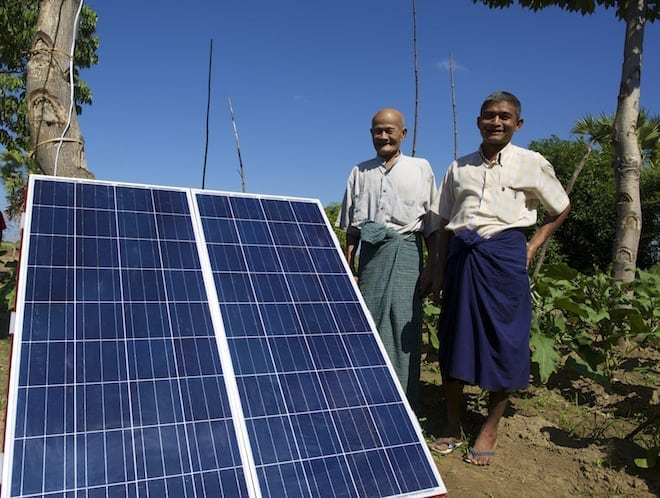
\includegraphics[width=0.9\textwidth]{Docs/lotus-solar-pump}
  \end{figure}
\end{frame}

\begin{frame}{Antes de empezar!!!!}{El elefante en la habitación.}
  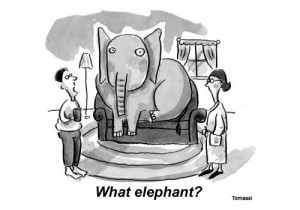
\includegraphics{Docs/elefant_in_room}
\end{frame}

\begin{frame}{Antes de empezar!!!!}{El elefante en la habitación.}
  \textbf{¿Cómo puede un agricultor adoptar estas tecnologías?}
  Tomando en consideración:
  \begin{itemize}
    \item El precio de esta tecnología.
    \item La curva de aprendizaje
    \item Falta de infraestructura para aplicarlas (La electricidad es parte importante de un componente electrónico....)
  \end{itemize}
\end{frame}

\begin{frame}{¿Cuanto cuesta en realidad?}{La ley de Moore sigue vigente.}
  \begin{figure}
    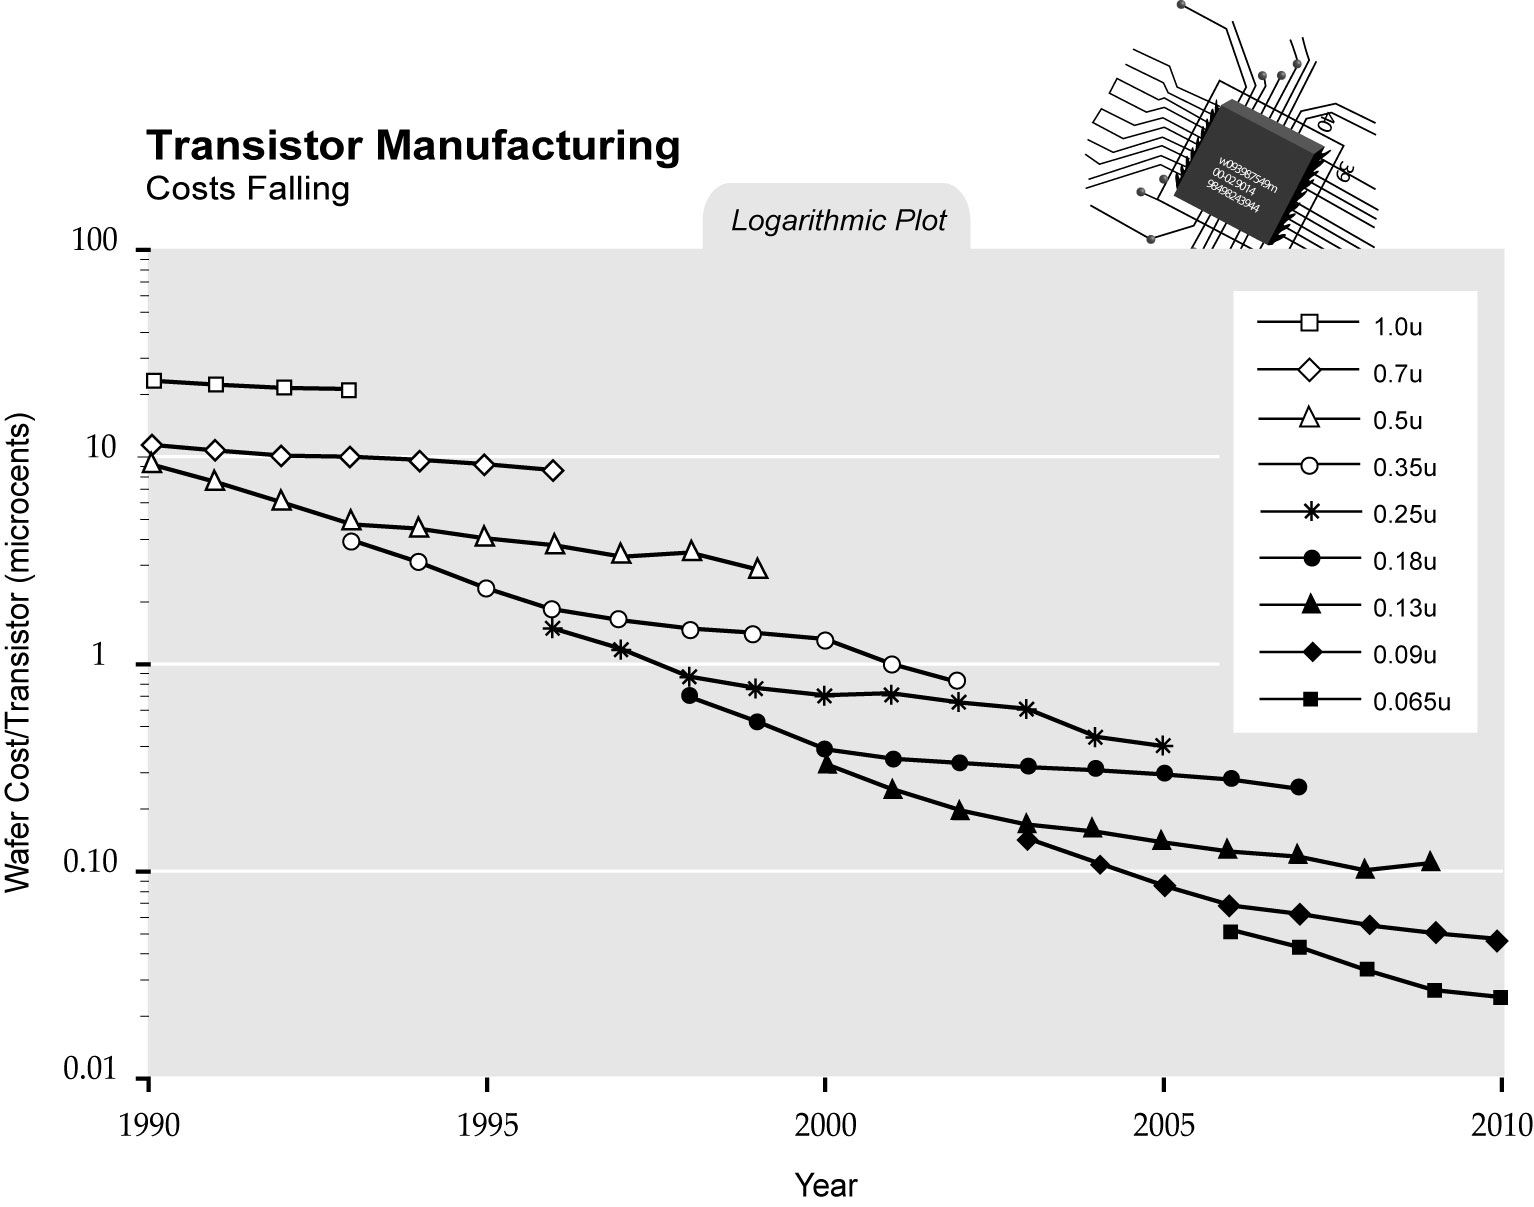
\includegraphics[width=0.8\textwidth]{Docs/Trans_price}
    \caption{\tiny Randall Goodall, D. Fandel, and H.Huff, “Long-Term Productivity Mechanisms of the Semiconductor Industry,” Ninth International Symposium on Silicon Materials Science and Technology, }
    \label{Moore_law}
  \end{figure}
\end{frame}

\begin{frame}
    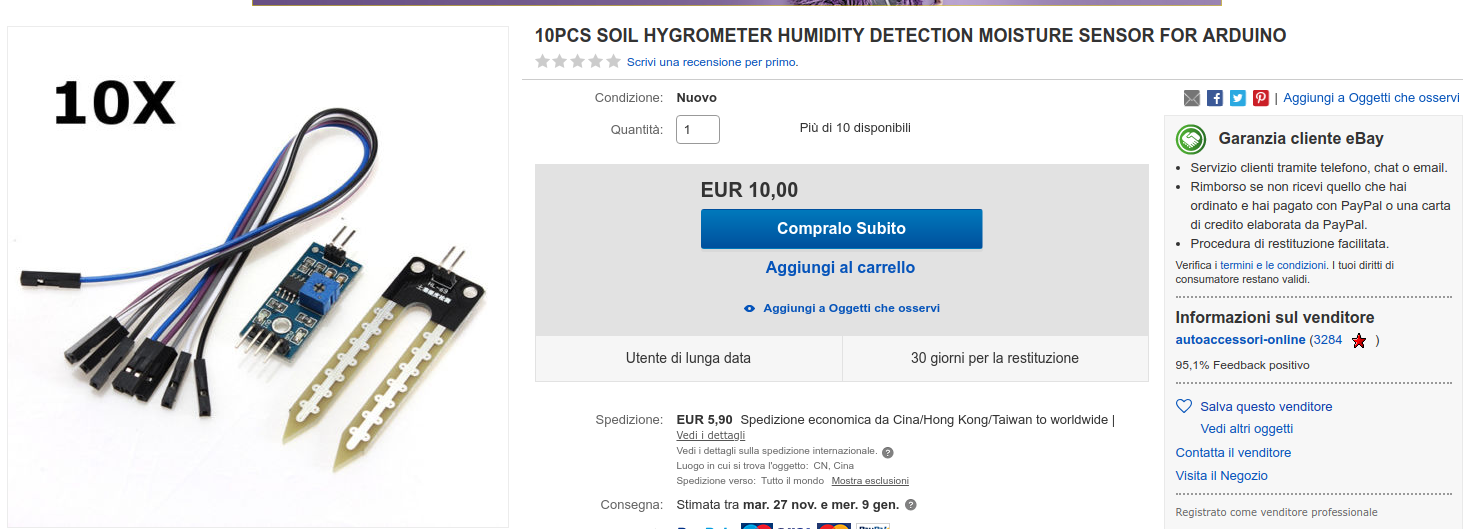
\includegraphics[width=\textwidth]{Docs/soil_humidity}
\end{frame}

\begin{frame}{No es tan difícil}{Si está bien diseñado}
  \begin{columns}
    \begin{column}{0.5\textwidth}
      \center
      \textbf{Curva de aprendizaje del programador:}

      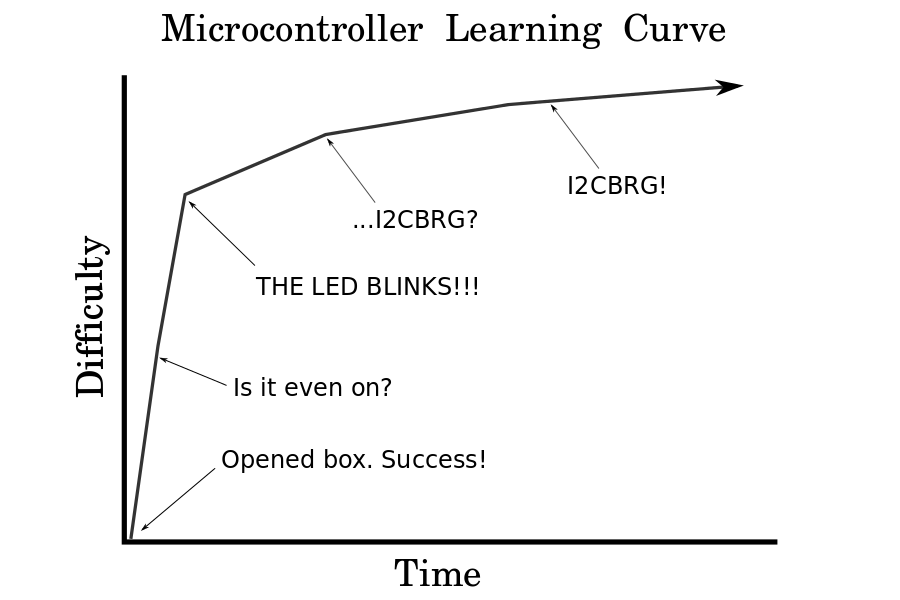
\includegraphics[width=\textwidth]{Docs/micro_lc}
    \end{column}
    \begin{column}{0.5\textwidth}
      \center
      \textbf{Curva de aprendizaje del usuario:}

      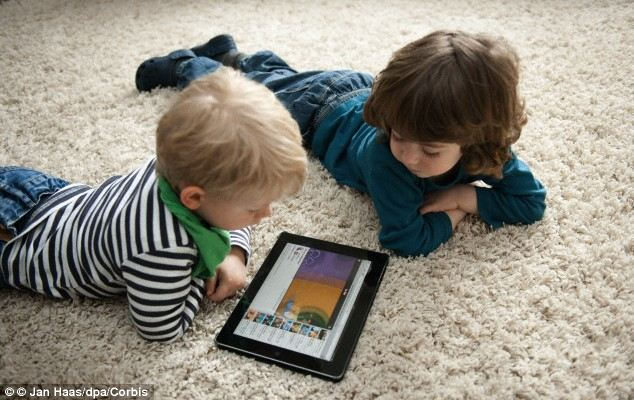
\includegraphics[width=\textwidth]{Docs/baby_tablet}
    \end{column}
\end{columns}
\end{frame}

\begin{frame}{}
  \begin{columns}
    \begin{column}{0.7\textwidth}
      \begin{figure}
        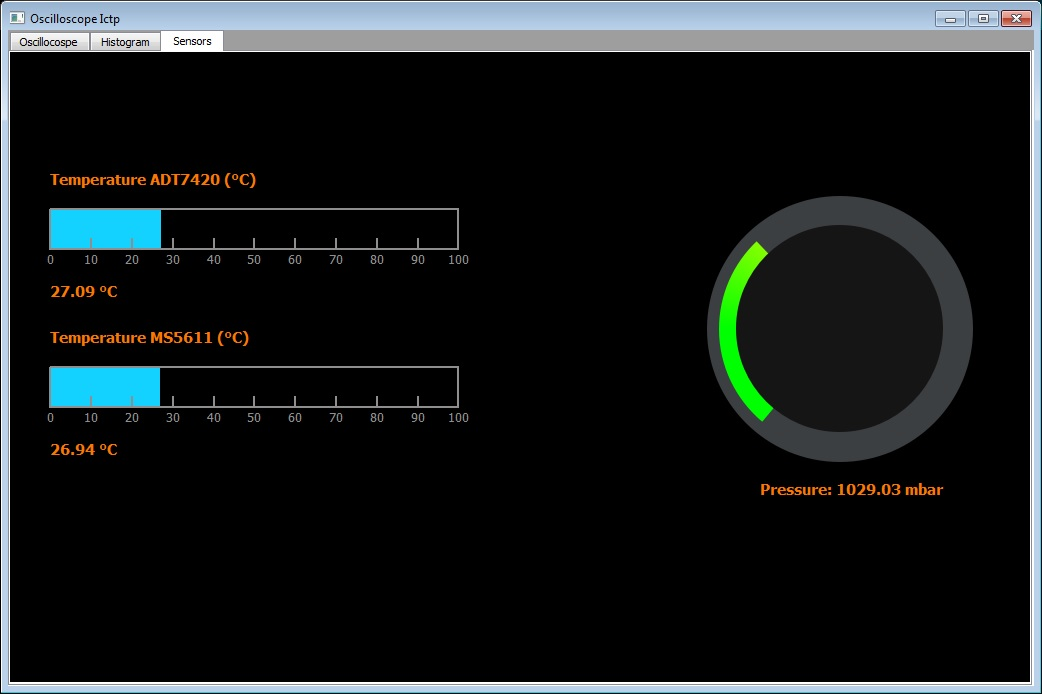
\includegraphics[width=\textwidth]{Docs/sensorfinal}
        \caption{Interfáz gráfica realizada en PyQT para interacción con sensores}
        \label{}
      \end{figure}
    \end{column}
    \begin{column}{0.3\textwidth}
      \begin{figure}
        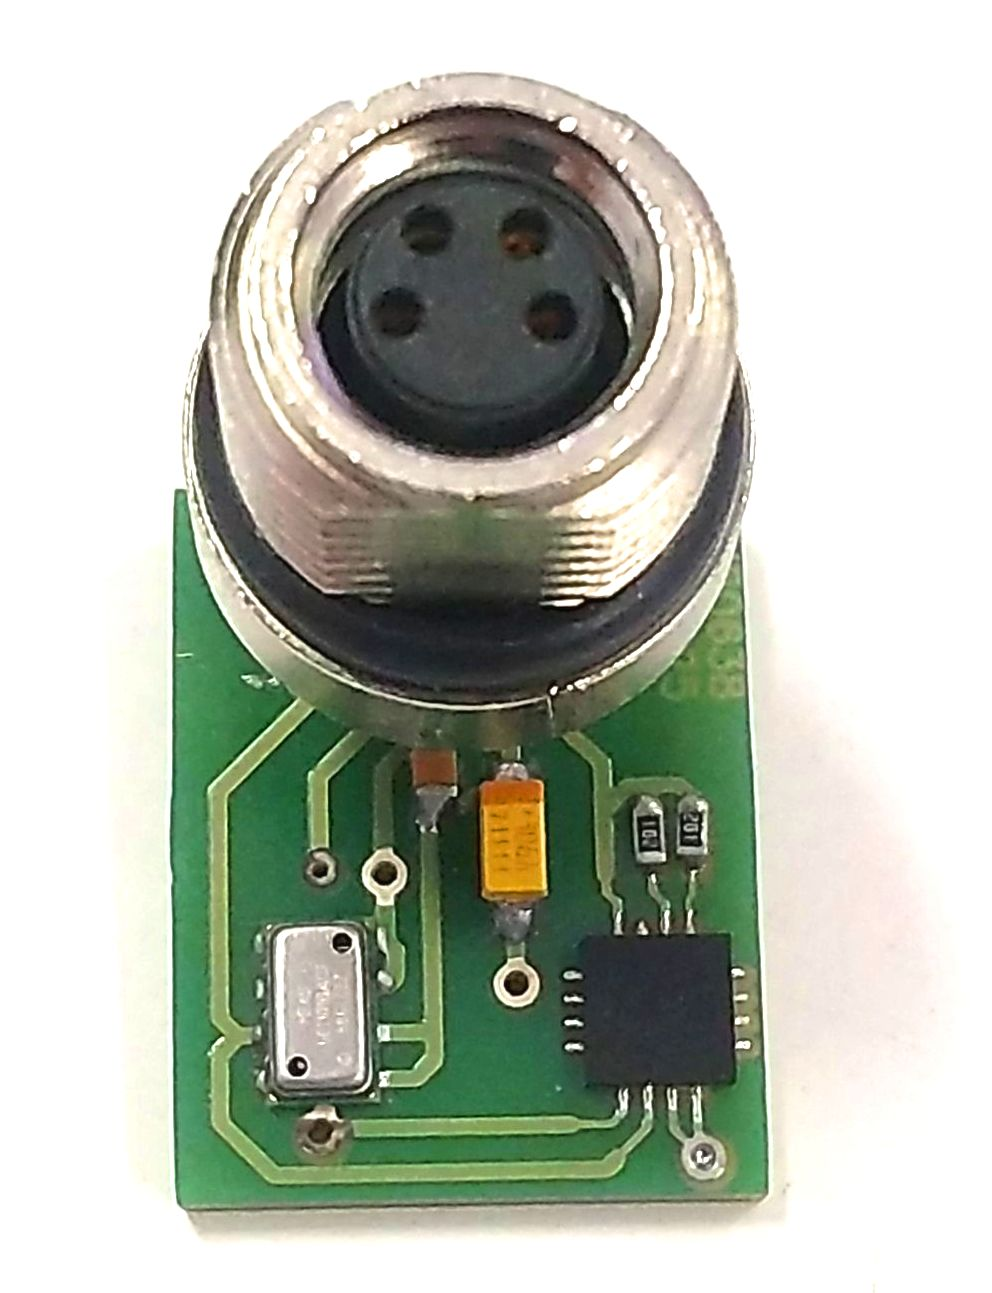
\includegraphics[width=\textwidth]{Docs/Temppress}
        \caption{Sensores de temperatura y presion atmosférica para medición de precisión en gases.}
        \label{}
      \end{figure}
    \end{column}
  \end{columns}
\end{frame}

\begin{frame}{Red de cobertura celular en Guatemala}
  \begin{figure}
    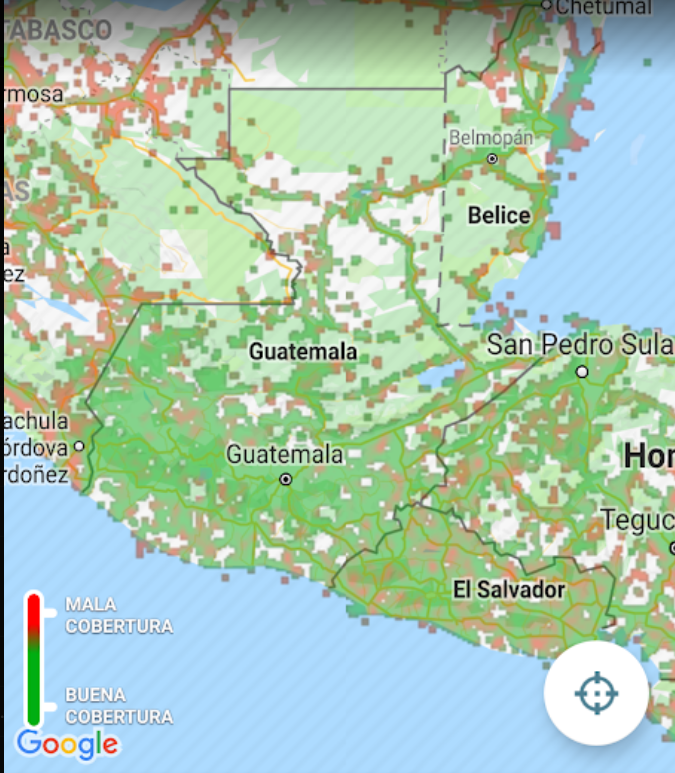
\includegraphics[height=0.75\textheight]{Docs/opensky}
    \caption{Cobertura celular de compañias Claro, Tigo y Movistar en bandas 2G, 3G y 4G.
    \emph{Fuente:www.opensignal.com}}
    \label{}
  \end{figure}
\end{frame}

\subsection{Tipos de instrumentación electrónica}
\begin{frame}{Tipos de instrumentación electrónica}
  \center
  Una tecnología solamente es tan buena como la persona que la aplica.
\end{frame}

\begin{frame}{Tipos de instrumentación electrónica}{Clasificación por precio}

  Según el costo o la complejidad de la instrumentación a utiliar, esta la podemos catalogar en cuatro gamas distintas:
  \begin{itemize}
    \item Baja
    \item Media
    \item Alta
    \item Experimental
  \end{itemize}
\end{frame}

\begin{frame}{Tipos de instrumentación electrónica}{Clasificación por precio}
  Según el costo o la complejidad de la instrumentación a utiliar, esta la podemos catalogar en cuatro gamas distintas:
  \begin{itemize}
    \item \textbf{Baja:}

      Pequeños agricultores y personas partículares
    \item \textbf{Media:}

      Cooperativas, Empresas privadas

    \item \textbf{Alta:}

      Comisiones departamentales, Estado de Guatemala.
    \item \textbf{Experimental:}

      Investigadores, Universidades
  \end{itemize}
\end{frame}

\section{Aplicaciones específicas en cada gama}

\subsection{Gama Baja}

\begin{frame}{Ejemplos de Gama Baja}{\emph{The Chameleon}}
  \begin{figure}
    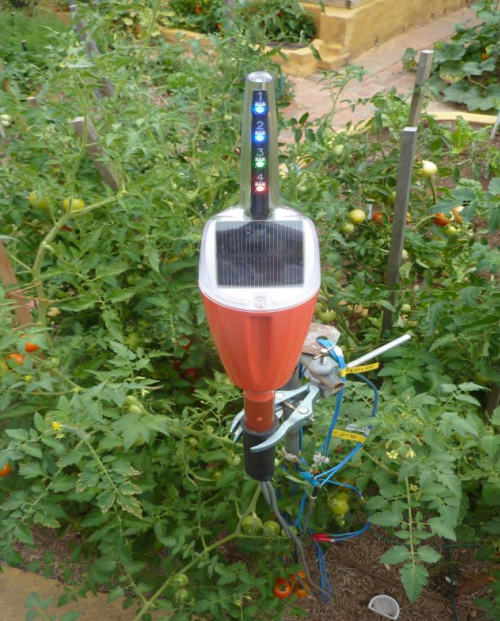
\includegraphics[width=0.7\textwidth]{Docs/chameleon1}
    \caption{}
    \label{}
  \end{figure}

\end{frame}

\begin{frame}{Ejemplos de Gama Baja}{\emph{The Chameleon}}
  Higrómetro de tensión digital basado en sensor resistivo con interfáz simple para medición de la humedad del suelo en Mozambique.

  Ventajas:
  \begin{itemize}
    \item Interfáz simple de comprender y enseñar.
    \item Fácil instalación in-situ
    \item Uso de componentes pasivos hace fácil de réplicar.
  \end{itemize}

  Desventajas:
  \begin{itemize}
    \item Requiere precalibración
    \item Humedad limitada a un tipo de suelo en partícular.
  \end{itemize}
\end{frame}
\begin{frame}{Ejemplos de Gama Baja}{\emph{The Chameleon}}
  \begin{figure}
    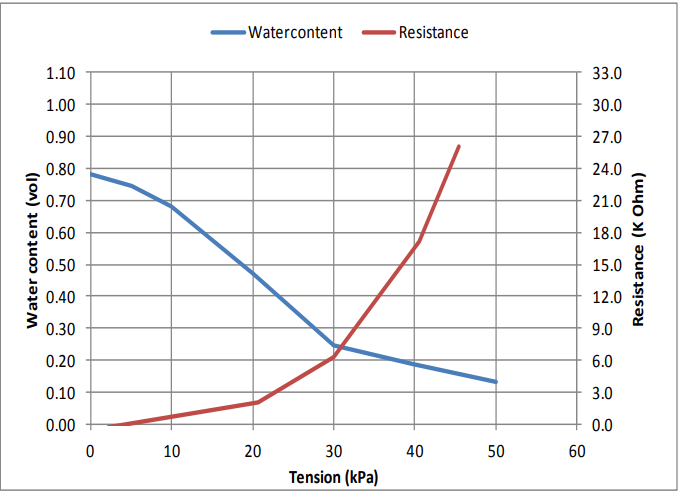
\includegraphics[width=0.7\textwidth]{Docs/chameleon2}
    \caption{Relación entre tensión, humedad y resistencia.}
    \label{}
  \end{figure}
\end{frame}

\begin{frame}{Ejemplos de Gama Baja}{\emph{The Chameleon}}
  \begin{figure}
    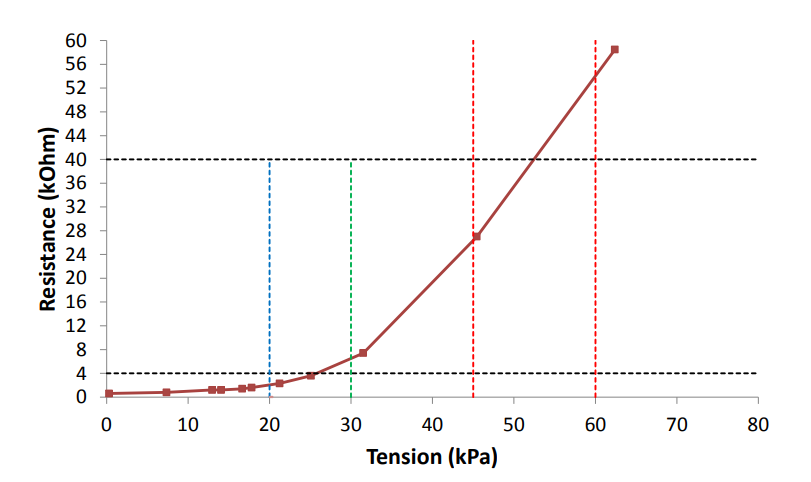
\includegraphics[width=0.7\textwidth]{Docs/chameleon3}
    \caption{Delimitación de los indicadores de humedad según valores de tensión.}
    \label{}
  \end{figure}
\end{frame}

\begin{frame}{Ejemplos de Gama Baja}{\emph{The Chameleon}}
  \begin{figure}
    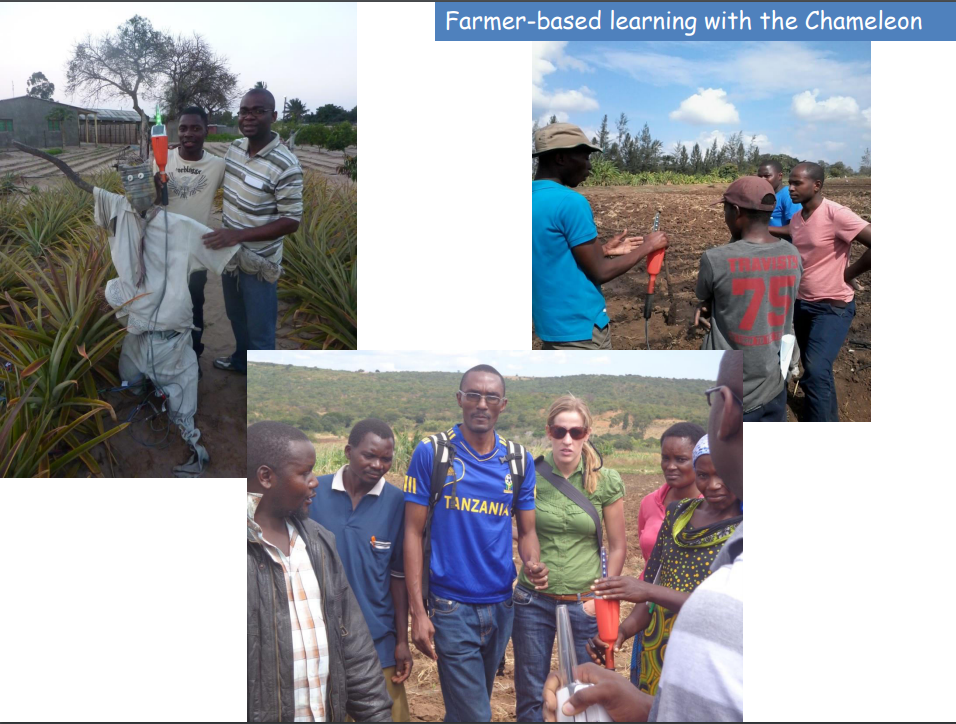
\includegraphics[width=\textwidth]{Docs/chameleon4}
  \end{figure}
\end{frame}


\begin{frame}{Ejemplos de Gama Baja}{Groasis}
  \begin{figure}
    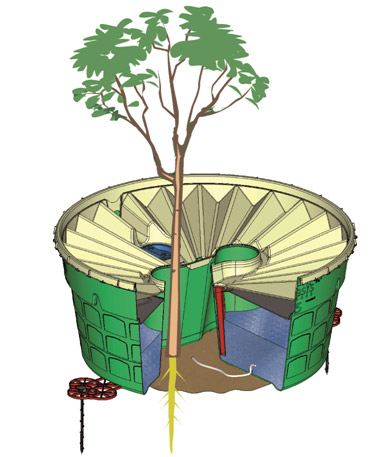
\includegraphics[width=0.6\textwidth]{Docs/groasis1}
  \end{figure}
\end{frame}

\begin{frame}{Ejemplos de Gama Baja}{Groasis}

Caja de polypropyleno reutilizable a usarse como alternativa a riego por goteo para la fase de crecimiento en cultivos arbóreos. Disponible con sensores te humedad en el suelo para optimizar la liberación del agua.
  Ventajas:
  \begin{itemize}
    \item Reutilizable (Hasta 10 veces según documentación)
    \item Ahorro de hasta 90 porciento de agua en riego con goteo.
    \item Permite la captación de agua debido a su diseño.
  \end{itemize}

  Desventajas:
  \begin{itemize}
    \item Costo relativamente caro.
    \item No es un proyecto abierto.
    \item Documentación sobre los sensores no disponible.
  \end{itemize}
\end{frame}


\begin{frame}{Ejemplos de Gama Baja}{Burried Diffuser}{Difusor enterrado}
  \begin{figure}
    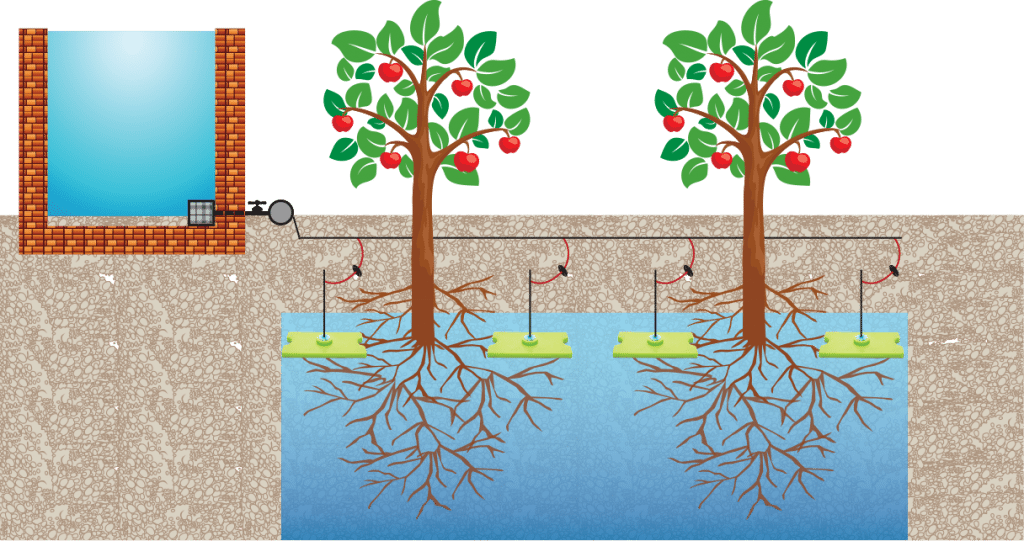
\includegraphics[width=0.6\textwidth]{Docs/bd1}
  \end{figure}

\end{frame}

\subsection{Gama Media}
\begin{frame}{Gama Media}{3D-PAWS}
  \begin{figure}
    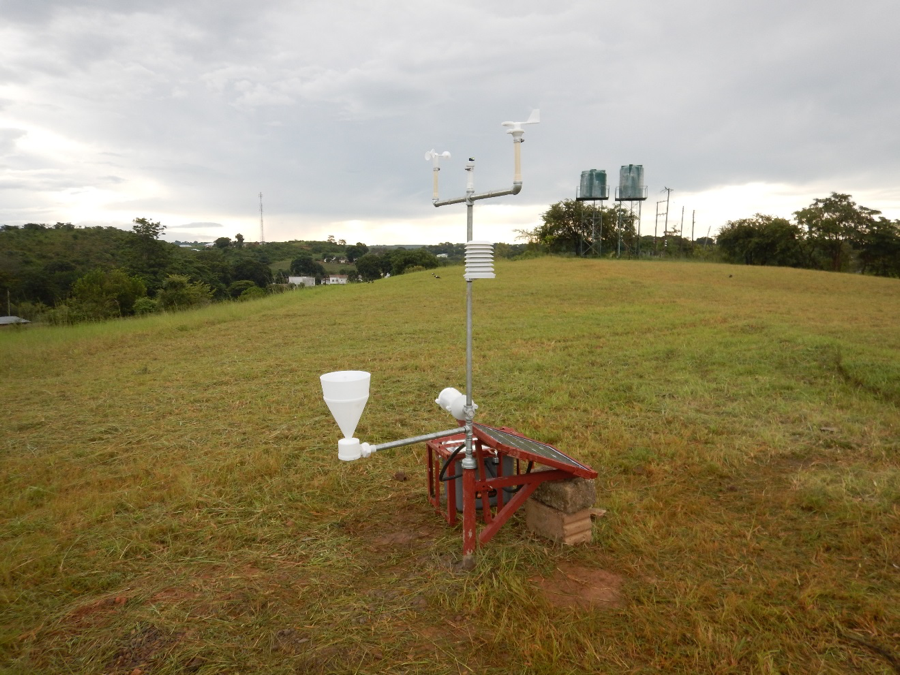
\includegraphics[height=0.7\textheight]{Docs/3dpaws1}
    \caption{3D-PAWS location at the Bio-Med College at the Salvation Army Mission, Zambia.}
  \end{figure}
\end{frame}

\begin{frame}{Gama Media}{3D-PAWS}
\emph{3D Printed Automatic Weather Station}, tiene como objetivo el proporcionar una estación metereológica "Personal" para contar con datos confiables sobre las condiciones climáticas. Todos los componentes pueden ser manufacturados en una semana y tiene un costo entre 200 USD a 400 USD.

Consta con los siguientes sensores:
\begin{itemize}
  \item Presión
  \item Humedad relativa.
  \item Temperatura.
  \item Velocidad del viento.
  \item Dirección del viento.
  \item Precipitación pluvial.
  \item Intensidad de luz visible, infraroja y UV.
\end{itemize}

\end{frame}

\begin{frame}{Gama Media}{3D-PAWS}
El sistema está basado en una Raspberry Pi para la adquisición de datos, procesamiento y comunicaciónes.

\begin{figure}
  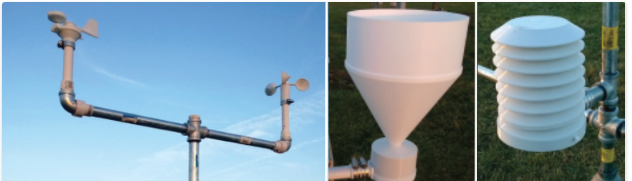
\includegraphics[height=0.4\textheight]{Docs/3dpaws2}
  \caption{Anemometro y veleta, Pluviometro y Radiation shield impresos en 3d.}
  \label{}
\end{figure}
\end{frame}

\subsection{Gama Alta}
\begin{frame}{Ejemplos de Gama Alta}{Sonda de Neutrones}
  \begin{figure}
    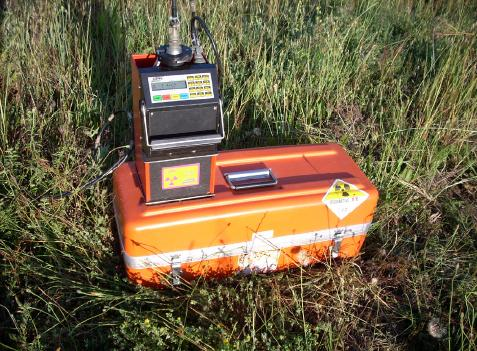
\includegraphics[height=0.7\textheight]{Docs/sondaneutrones}
    \caption{Sonda de neutrones CPN 503-DR Hydroprobe en posición de conteo estándar y medición en el suelo. }
    \label{}
  \end{figure}

\end{frame}

\begin{frame}{Ejemplos de Gama Alta}{Sonda de Neutrones}
Es uno de los dispositivos para medición de humedad más confiables. Usualmente consta de una fuente de neutrones rápidos y de un detector de neutrones lentos. Usualmente la fuente de neutrones es una fuente de Berilio ($^{10}Be$) que emite neutrones en todas direcciones. Estos neutrones chocan con los átomos del suelo y rebotan perdiendo energía haciendo que se vuelvan "lentos". La interacción con la molécula del agua (en especial el hidrógeno) hace que se forme una nube de neutrones lentos los cuales son contados con el detector.

\begin{figure}
  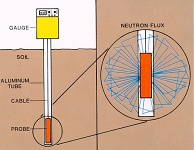
\includegraphics[height=0.4\textheight]{Docs/sondaneutrones2}
  \caption{Representación de la fuente radiactiva en el suelo.}
  \label{}
\end{figure}

\end{frame}

\begin{frame}{Ejemplos de Gama Alta}{Sonda de Neutrones}
Ventajas:

\begin{itemize}
  \item Dispositivo de alta precisión y exactitud.
  \item Funciona con cualquier tipo de suelo, incluso congelado.
  \item Uso sencillo.
\end{itemize}

Desventajas:
\begin{itemize}
   \item Se necesita una fuente radioactiva.
   \item Costo alto
   \item Necesita cumplir con licencias y regulaciones de uso.
\end{itemize}

\end{frame}

% \begin{frame}{Ejemplos de Gama Alta}{Monitoreo Satelital}
%   \begin{figure}
%     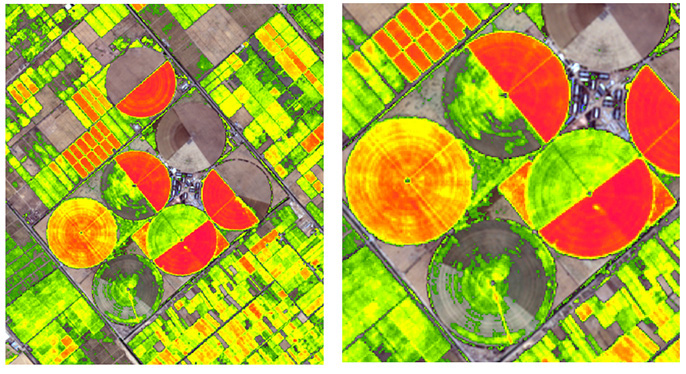
\includegraphics[height=0.7\textheight]{Docs/ms1}
%     \caption{}
%     \label{}
%   \end{figure}
% \end{frame}


\subsection{Experimental}
\begin{frame}{Ejemplos Experimentales}{Fibra Óptica}
  \begin{figure}
    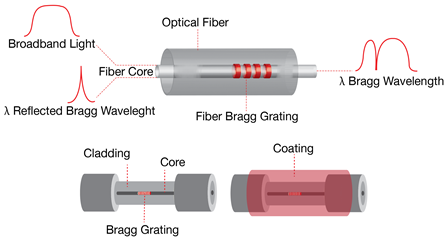
\includegraphics[height=0.7\textheight]{Docs/exp1}
    \caption{}
    \label{}
  \end{figure}

\end{frame}

\begin{frame}{Ejemplos Experimentales}{Fibra Óptica}
  \begin{figure}
    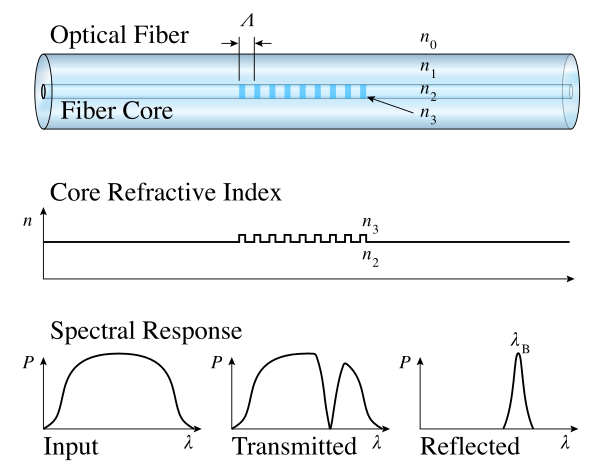
\includegraphics[height=0.7\textheight]{Docs/exp2}
    \caption{}
    \label{}
  \end{figure}

\end{frame}

\begin{frame}{Ejemplos Experimentales}{Fibra Óptica}
  \begin{figure}
    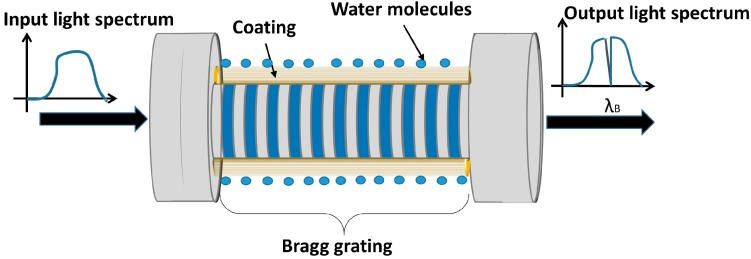
\includegraphics[width=0.7\textwidth]{Docs/exp3}
    \caption{Schematic of an optical fiber humidity sensor using fiber Bragg gratings.}
    \label{}
  \end{figure}

\end{frame}

\begin{frame}{Ejemplos Experimentales}{Fibra Óptica}
  \begin{figure}
    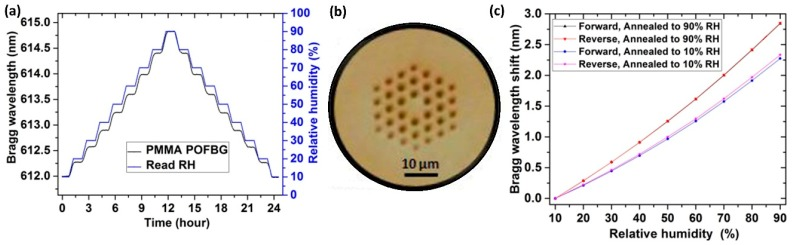
\includegraphics[width=\textwidth]{Docs/exp4}
    \caption{(a) Measured humidity response at 25 °C of PMMA mPOFBG annealed up to 90\%RH versus time and humidity; (b) Microscope image of the end facet of PMMA mPOF; (c) Corresponding stabilized response of the PMMA mPOFBGs annealed up to 90\% and 10\%.}
    \label{}
  \end{figure}

\end{frame}



\end{document}
